\documentclass{article}

\usepackage{graphicx}
\usepackage{tikz}
\usepackage{tikzsymbols}
\usetikzlibrary{calc,patterns,shapes.geometric}
\pagestyle{empty}
\usepackage[margin=0pt]{geometry}
\geometry{papersize={14in,12in}}

\def\centerarc[#1](#2)(#3:#4:#5){\draw[#1] ($(#2)+({#5*cos(#3)},{#5*sin(#3)})$) arc (#3:#4:#5);}

\begin{document}
	\begin{figure}
		\centering
		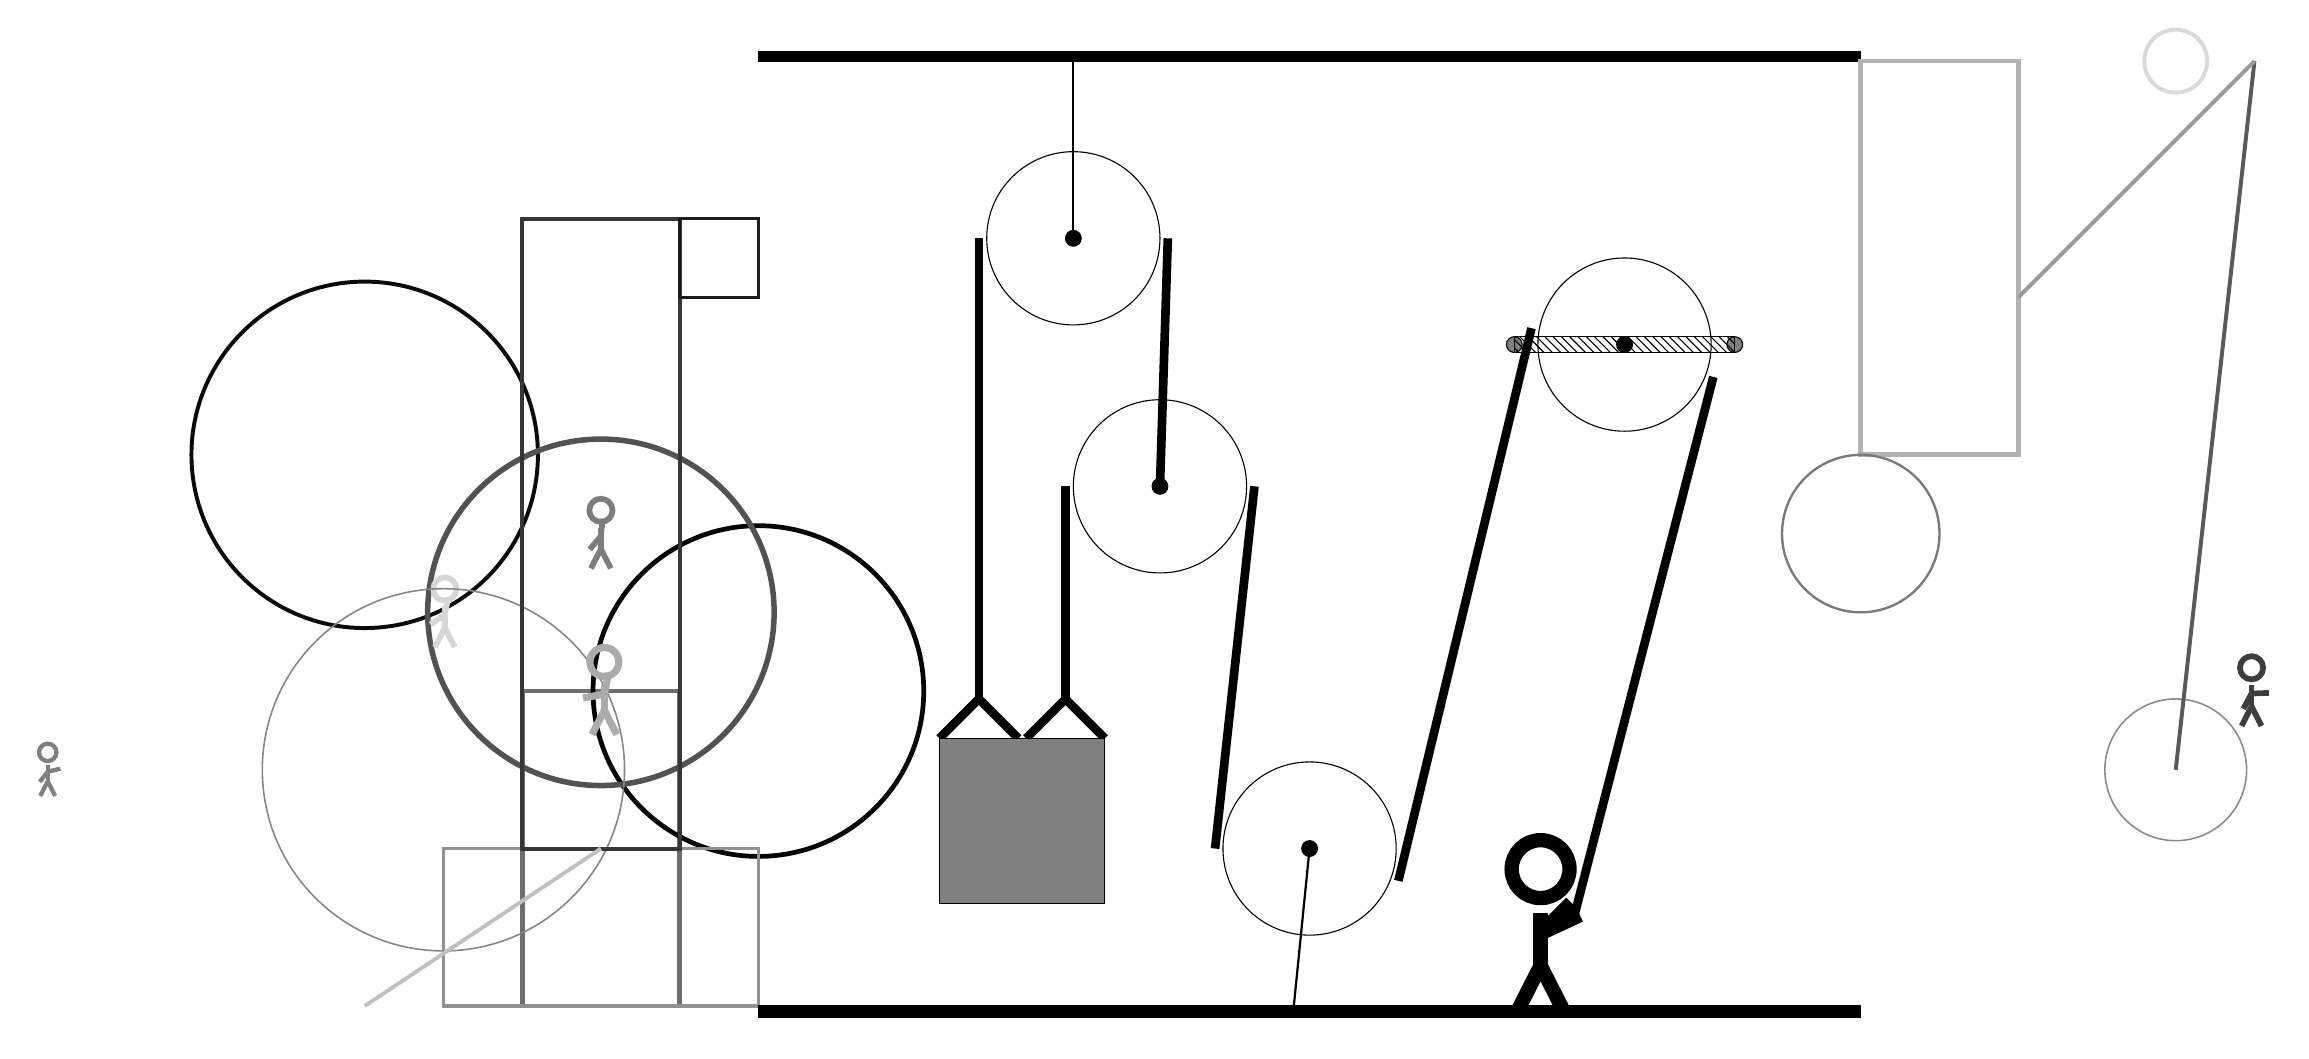
\begin{tikzpicture}
			%%%%% START %%%%%
			
			\draw[fill=black] (-2, 9) rectangle (12, 9.125);
			
			\draw (2, 6.75) circle (1.1);
			\draw[fill=black] (2, 6.75) circle (0.1);
			\draw[thick] (2, 6.75) -- (2, 9);
			
			\draw (3.1, 3.6) circle (1.1);
			\draw[fill=black] (3.1, 3.6) circle (0.1);
			
			\draw (5, -1) circle (1.1);
			\draw[fill=black] (5, -1) circle (0.1);
			\draw[thick] (5, -1) -- (4.8, -3);
			
			\draw (9, 5.4) circle (1.1);
			\draw[fill=black] (9, 5.4) circle (0.1);
			\draw[fill=black!50] (7.6, 5.4) circle (0.1);
			\draw[fill=black!50] (10.4, 5.4) circle (0.1);
			\draw[pattern=north west lines, pattern color=black] (7.6, 5.5) rectangle (10.4, 5.3);
			
			\draw[line width = 1.1mm]  (0.3, 0.4) -- (0.8, 0.9) -- (1.3, 0.4);
			\draw[line width = 1.1mm]  (1.4, 0.4) -- (1.9, 0.9) -- (2.4, 0.4);
			\draw[fill=black!50] (0.3, 0.4) rectangle (2.4, -1.7);
			
			\draw[line width=0.6mm, color=black!30] (14, 4) rectangle (12, 9);
			
			\draw[line width=0.6mm, color=black!57] (-3, 1) rectangle (-5, -3);
			\draw [line width=0.2mm, color=black!46](16, 0) circle (0.9);
			\draw [line width=0.6mm, color=black!98](-2, 1) circle (2.1);
			
			\draw [line width=0.5mm, color=black!96](-7, 4) circle (2.2);
			\draw [line width=0.7mm, color=black!68](-4, 2) circle (2.2);
			\node[line width=0.2mm, color=black!51] at (-4, 3) {\Strichmaxerl[4][50][84]};
			\draw [line width=0.6mm, color=black!48](15, 8) circle (0.0);
			\draw[line width=0.5mm, color=black!65](17, 9) -- (16, 0);
			\node[line width=0.4mm, color=black!16] at (-6, 2) {\Strichmaxerl[4][34][79]};
			\draw [line width=0.2mm, color=black!48](-6, 0) circle (2.3);
			\draw[line width=0.3mm, color=black!65] (-4, 3) rectangle (-4, 3);
			\node[line width=0.2mm, color=black!76] at (17, 1) {\Strichmaxerl[4][62][2]};
			
			\node[line width=0.4mm, color=black!33] at (-4, 1) {\Strichmaxerl[5][10][79]};
			\draw[line width=0.4mm, color=black!43] (-2, -1) rectangle (-6, -3);
			\draw[line width=0.5mm, color=black!79] (-3, -1) rectangle (-5, 7);
			
			\draw [line width=0.3mm, color=black!52](12, 3) circle (1.0);
			\draw [line width=0.5mm, color=black!15](16, 9) circle (0.4);
			\node[line width=0.7mm, color=black!50] at (-11, 0) {\Strichmaxerl[3][52][13]};
			
			\draw[line width=0.3mm, color=black!89] (-2, 6) rectangle (-3, 7);
			\draw[line width=0.5mm, color=black!25](-4, -1) -- (-7, -3);
			
			\draw[line width=0.5mm, color=black!40](14, 6) -- (17, 9);
			
			\draw[line width = 1.1mm] (0.8, 6.75) -- (0.8, 0.9);
			\centerarc[line width = 1.1mm](2, 6.75)(0:180:1.2000000000000002);
			\draw[line width = 1.1mm] (3.2, 6.75) -- (3.1, 3.6);
			\draw[line width = 1.1mm] (1.9, 3.6) -- (1.9, 0.9);
			\centerarc[line width = 1.1mm](3.1, 3.6)(0:180:1.2000000000000002);
			\draw[line width = 1.1mm] (4.3, 3.6) -- (3.8, -1);
			\centerarc[line width = 1.1mm](5, -1)(180:340:1.2000000000000002);
			\draw[line width=1.1mm](6.1276, -1.4104) -- (7.8182, 5.6083);
			\centerarc[line width = 1.1mm](9, 5.4)(-20:170:1.2000000000000002);
			\draw[line width=1.1mm](10.1276, 4.9896) --  (8.35, -1.9);
			
			\node at (8, -2) {\Strichmaxerl[10][225][25]};
			
			\draw[fill=black] (-2, -3) rectangle (12, -3.15);
			
			%%%%% END %%%%%
		\end{tikzpicture}
	\end{figure}	
\end{document}